%! Author = jahle
%! Date = 12.09.2025

% Preamble
\documentclass[11pt]{article}

% Packages
\usepackage{amsmath}
\usepackage{tcolorbox}


% Document
\begin{document}

\title{Assignment 2}
\author{Anders Emil Bergan \& Jens Martin Jahle}
\date{\today}

\maketitle
\tcbsubtitle{Exercise 1 - Sudoko Solver}

\begin{figure}[h!]
    \centering
    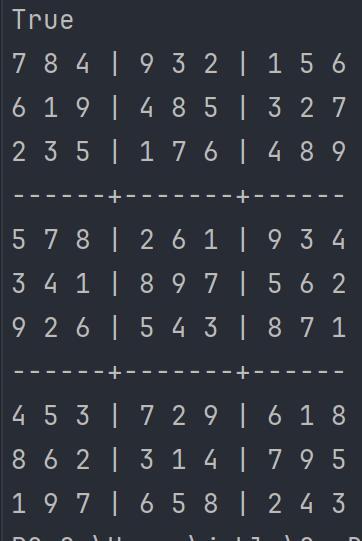
\includegraphics[width=0.6\textwidth]{images/sudoko_easy}
    \caption{Sudoko solution - Easy}
    \label{fig:easy}
\end{figure}

\begin{figure}[h!]
    \centering
    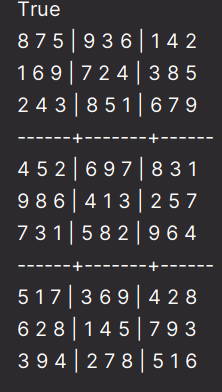
\includegraphics[width=0.6\textwidth]{images/sudoko_medium}
    \caption{Sudoko solution - Medium}
    \label{fig:medium}
\end{figure}

\begin{figure}[h!]
    \centering
    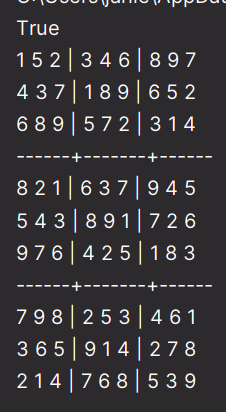
\includegraphics[width=0.6\textwidth]{images/sudoko_hard}
    \caption{Sudoko solution - Hard}
    \label{fig:hard}
\end{figure}

\begin{figure}[h!]
    \centering
    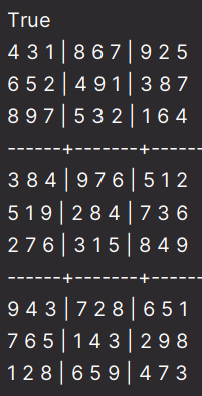
\includegraphics[width=0.6\textwidth]{images/sudoko_very_hard}
    \caption{Sudoko solution - Very Hard}
    \label{fig:very-hard}
\end{figure}




\end{document}